\section{Aufgaben}
Wesentliche Fragestellungen, welche in diesem Kapitel gelöst werden sollen, sind auf der einen Seite, welche vorhandene IT-Systeme bereits zentral Verwendung finden und auf der anderen Seite, wie Informationen bereits Repräsentiert werden. In dieser Analyse wird Aufschluss darüber gegeben, ob ein Informationsmanagement bereits an der Hochschule betrieben wird oder wie Informationen bereits zentral zur Verfügung gestellt werden. 
Bei der Hochschule Emden-Leer handelt es sich um eine kleine Hochschule mit aktuell 4626 eingeschriebenen Studierenden. Den größten Anteil machen die 4303 Studenten vor Ort aus.\footnote{\url{http://www.hs-emden-leer.de/fileadmin/user_upload/Einrichtungen/ZDF/Studierende/JV_Stud_20142.pdf}} Es sind 396 Mitarbeiter beschäftigt, wobei 107 Professuren sind.\footnote{\url{https://www.hs-emden-leer.de/no_cache/hochschule/zahlen-daten-fakten.html}}

Der wesentliche Bestandteil dieses Kapitels ist der Prozess der Sammlung, Selektion und Prüfung von Fragestellung, welche die Grundlage für ein Experten Interview bilden. Dieses Interview wurde von den Studierenden Tina Koppermann und Marc Enders sowie der betreuenden Professorin, Frau Prof. Dr. Krüger-Basener, mit dem Leiter des Hochschulzentrums Emden/Leer Herrn Günter Müller durchgeführt. 

Es wurde bei der Erstellung dieses Experten Interviews auf die Methodik des SPSS-Prinzips verstärkt reflektiert. Dem SPSS-Prinzip nach Helfferich\footnote{\cite{helfferich_2009}} liegt folgendes Vorgehen zur Grunde:
\begin{enumerate}
	\item Sammeln
	\item Prüfen
	\item Selektieren
	\item Subsumieren		
\end{enumerate}
Mit Hilfe von diesem Prinzip zur qualitativen Datenerhebung werden im ersten Schritt Fragen gesammelt. Diese konnten von allen Kursteilnehmern in einem zur Verfügung gestellten Online-Dokument eingesehen und editiert werden. Bei der Sammlung der Fragen wurden insgesamt 62 Fragestellungen zu unterschiedlichen Schwerpunkten aufgenommen.

In Abbildung \ref{fig_auszug_fragen_sammeln} ist ein Auszug aus dem entwickelten Fragenkatalog wiedergegeben.
\begin{figure}[h!]
	\centering
	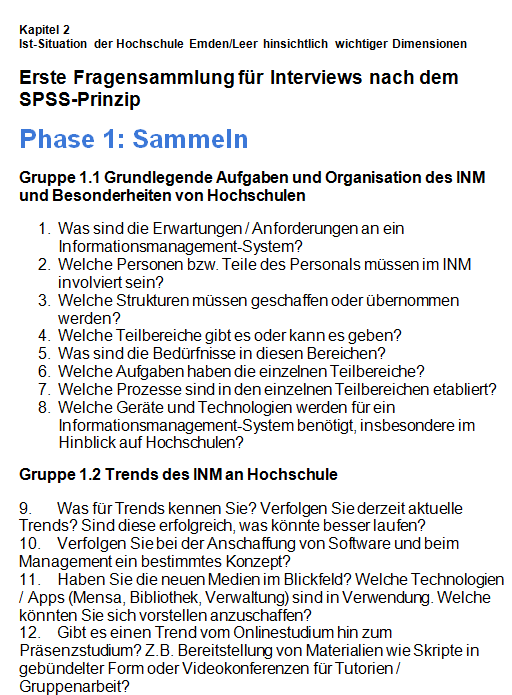
\includegraphics[width=10cm]{kapitel/gruppe2/bilder/auszug_fragen}
	\caption{Auszug der gesammelten Fragen}
	\label{fig_auszug_fragen_sammeln}
\end{figure}
Nach der erfolgten Sammlung aller Fragen folgte im zweiten Schritt die Prüfung der Fragen. Hierbei wurden Fragen, welche offen gestellt wurden, aussortiert. Nach der erfolgreichen Prüfung der Fragen folgte im nächsten Schritt die Selektion von diesen. Es wurden die Fragegestellungen entsprechend Themengebieten zugeordnet und zusammengestellt. Im letzten Schritt, dem Subsumieren des SPSS-Prinzips, wurde für jedes Themengebiet eine Erzähl Aufforderung gefunden und der Interviewleitfaden entsprechend diesen Erzähl Aufforderungen gegliedert. Mit Hilfe eines Farbcodes (siehe Abbildung \ref{fig_farbcode_SPSS}) wurden die Fragen entsprechend nach Erzähl Aufforderung, Checkliste, konkreter Frage und Aufrechterhaltungsfrage farblich markiert und anschließend einsortiert.

\begin{figure}[h!]
	\centering
	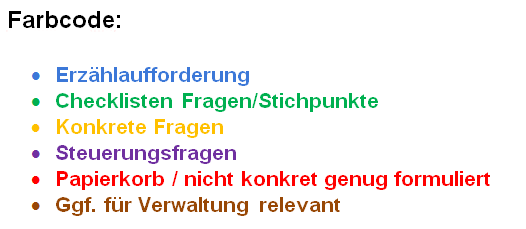
\includegraphics[width=10cm]{kapitel/gruppe2/bilder/farbcode_spss}
	\caption{angewandter Farbcode für das SPSS-Prinzip}
	\label{fig_farbcode_SPSS}
\end{figure}

\begin{figure}[h!]
	\centering
	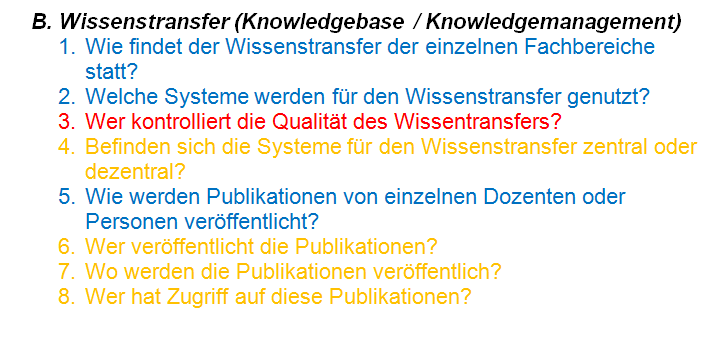
\includegraphics[width=10cm]{kapitel/gruppe2/bilder/sortierung_fragentyp}
	\caption{Sortierung der Fragen nach Fragentyp}
	\label{fig_sortierung_fragentyp}
\end{figure}

Diese Subsumierung wurde mit Hilfe des Anwendungsprogramms Microsoft Excel entsprechend visualisiert. Als Endergebnis  ist ein Interviewleitfaden entstanden, der in acht unterschiedliche Themenbereiche unterteilt wurde.

\begin{figure}[h!]
	\centering
	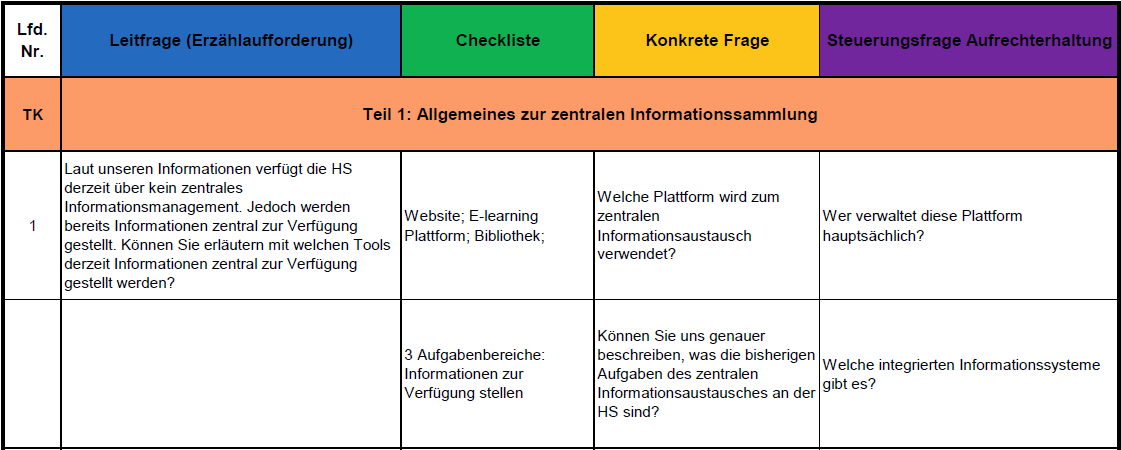
\includegraphics[width=10cm]{kapitel/gruppe2/bilder/auszug_leitfaden}
	\caption{Auszug des Interviewleitfadens}
	\label{fig_auszug_interviewleitfaden}
\end{figure}

An dem festgelegtem Interviewtermin ist mit Hilfe von diesem Leitfaden das Experten Interview mit Herrn Günter Müller, dem Leiter des Hochschulrechenzentrums an der Fachhochschule Emden/Leer, durchgeführt worden. Dieses Interview fand mit der Online Video Plattform „Adobe Connect“ statt und wurde mit Zustimmung von Herrn Müller digital aufgezeichnet. Im Anschluss an das Experten Interview wurde in der ersten Phase das Video auf wichtige inhaltliche Aspekte analysiert.

In der zweiten Phase wurde durch Transkription die digitale Aufzeichnung, mit Hilfe von der Applikation „Microsoft Word“, überführt. Mit dem Ziel die im Interview genannten Informationen besser verarbeiten zu können.

In der darauffolgenden Phase wurden mit Hilfe des Tools „Xmind“ zu jedem Themenbereich Mindmaps generiert, um bei der Recherche schneller auf Besonderheiten eingehen zu können.

Die Ergebnisse dieser IST-Analyse werden in den folgenden Kapiteln detaillierter beschrieben. 
